% !TEX root = ../main.tex
\chapter{Marco de referencia}

Este capítulo presenta los conceptos necesarios para interpretar el diseño
experimental. Primero se describe la patología digital y la relación entre
aprendizaje supervisado y no supervisado; luego se introducen las redes
convolucionales, la atención para aprendizaje de instancias múltiples y las
convoluciones equivariantes utilizadas en el VAE-\(\mathrm{SO}(2)\).

\section{Patología digital}

La patología digital reúne los sistemas usados para adquirir, almacenar,
visualizar y analizar portaobjetos en formato digital. Su elemento central es
la imagen completa del portaobjetos (WSI, \emph{whole-slide image}), obtenida
al digitalizar la preparación histológica con resolución suficiente para
examinarla a diferentes aumentos. Este soporte facilita la consulta remota, la
gestión de archivos y el desarrollo de métodos computacionales sobre la lámina
completa~\cite{pallua_future_2020,song_artificial_2023,baxi_digital_2022}.

Las WSI permiten entrenar modelos que reconocen patrones morfológicos,
cuantifican regiones y relacionan la apariencia tisular con variables
diagnósticas o pronósticas. Estas herramientas se han estudiado en múltiples
órganos y tareas, desde la detección de lesiones hasta la predicción de
biomarcadores; sin embargo, su adopción clínica también depende de validación,
interoperabilidad, calidad de los datos y supervisión humana
~\cite{niazi_digital_2019,song_artificial_2023,verghese_computational_2023}.

Una WSI puede contener miles de millones de píxeles y regiones extensas sin
tejido relevante. Por ello, los modelos suelen procesarla como una colección
de parches: cada parche conserva detalle celular y sus coordenadas mantienen
la relación espacial con la lámina. Esta descomposición hace posible entrenar
redes con memoria acotada, pero introduce la necesidad de seleccionar tejido,
agregar información entre parches y evitar que una misma WSI quede repartida
entre entrenamiento y evaluación~\cite{wang_managing_2012,niazi_digital_2019}.

\section{Tipos de aprendizaje de máquina}

El aprendizaje de máquina estima, a partir de datos, los parámetros de una
función que se utilizará para predecir o describir observaciones nuevas. La
distinción entre aprendizaje supervisado, no supervisado y semisupervisado
depende principalmente de qué variables objetivo están disponibles durante el
ajuste~\cite{goodfellow_deep_2016,chapelle_semisupervised_2006}.

\paragraph{Aprendizaje supervisado.}

En aprendizaje supervisado se observan pares \((\mathbf x_i,y_i)\), donde
\(\mathbf x_i\) es una entrada y \(y_i\) es la etiqueta o respuesta que el
modelo debe predecir. En patología, la respuesta puede ser el diagnóstico de
una WSI, la clase de un parche o una máscara espacial elaborada por un experto.
La Figura~\ref{fig:labelled} muestra este último caso.

\begin{figure}[h!]
    \centering
    
\includegraphics[width=0.6\textwidth]{labelled.jpg}
   \caption{Imágenes histopatológicas anotadas para guiar una tarea
   supervisada. Las regiones marcadas proporcionan una respuesta espacial para
   cada imagen.}
    \label{fig:labelled}
\end{figure}

\paragraph{Aprendizaje no supervisado.}

En aprendizaje no supervisado se observan las entradas, pero no una respuesta
externa para cada ejemplo. El objetivo puede ser modelar la distribución de
los datos, agrupar observaciones o aprender una representación de menor
dimensión que conserve información de la entrada
~\cite{goodfellow_deep_2016}. Esta situación es relevante en patología porque
las anotaciones densas requieren trabajo experto. En una experiencia de
anotación de 200 WSI de colon y piel, el tiempo por lámina varió desde segundos
hasta varias horas según la tarea~\cite{lindman_annotations_2019}; este rango
ilustra por qué no debe suponerse que todas las WSI disponibles tendrán una
máscara exhaustiva.

\begin{figure}
\centering
\subcaptionbox{Cluster A}{
\includegraphics[width=0.55\textwidth]{cluster_A.jpg}}%
\hfill
\subcaptionbox{Cluster B}{
\includegraphics[width=0.45\textwidth]{cluster_B.jpg}}%
\hfill
\caption{Agrupación ilustrativa de imágenes similares sin usar una etiqueta
objetivo para cada imagen.}
\label{fig:clustering}
\end{figure}

\paragraph{Aprendizaje semisupervisado.}

El aprendizaje semisupervisado combina una población amplia sin etiquetas con
otra, usualmente menor, que sí las contiene
~\cite{chapelle_semisupervised_2006}. Una estrategia posible es aprender
primero una representación sin supervisión y entrenar después un predictor con
las etiquetas disponibles. La Figura~\ref{fig:semi-supervised} ilustra esa
separación. En esta tesis se siguió precisamente este esquema: los VAE se
ajustaron con reconstrucción de parches y, una vez congelados, sus espacios
latentes alimentaron las tareas supervisadas.

\begin{figure}[h!]
    \centering
    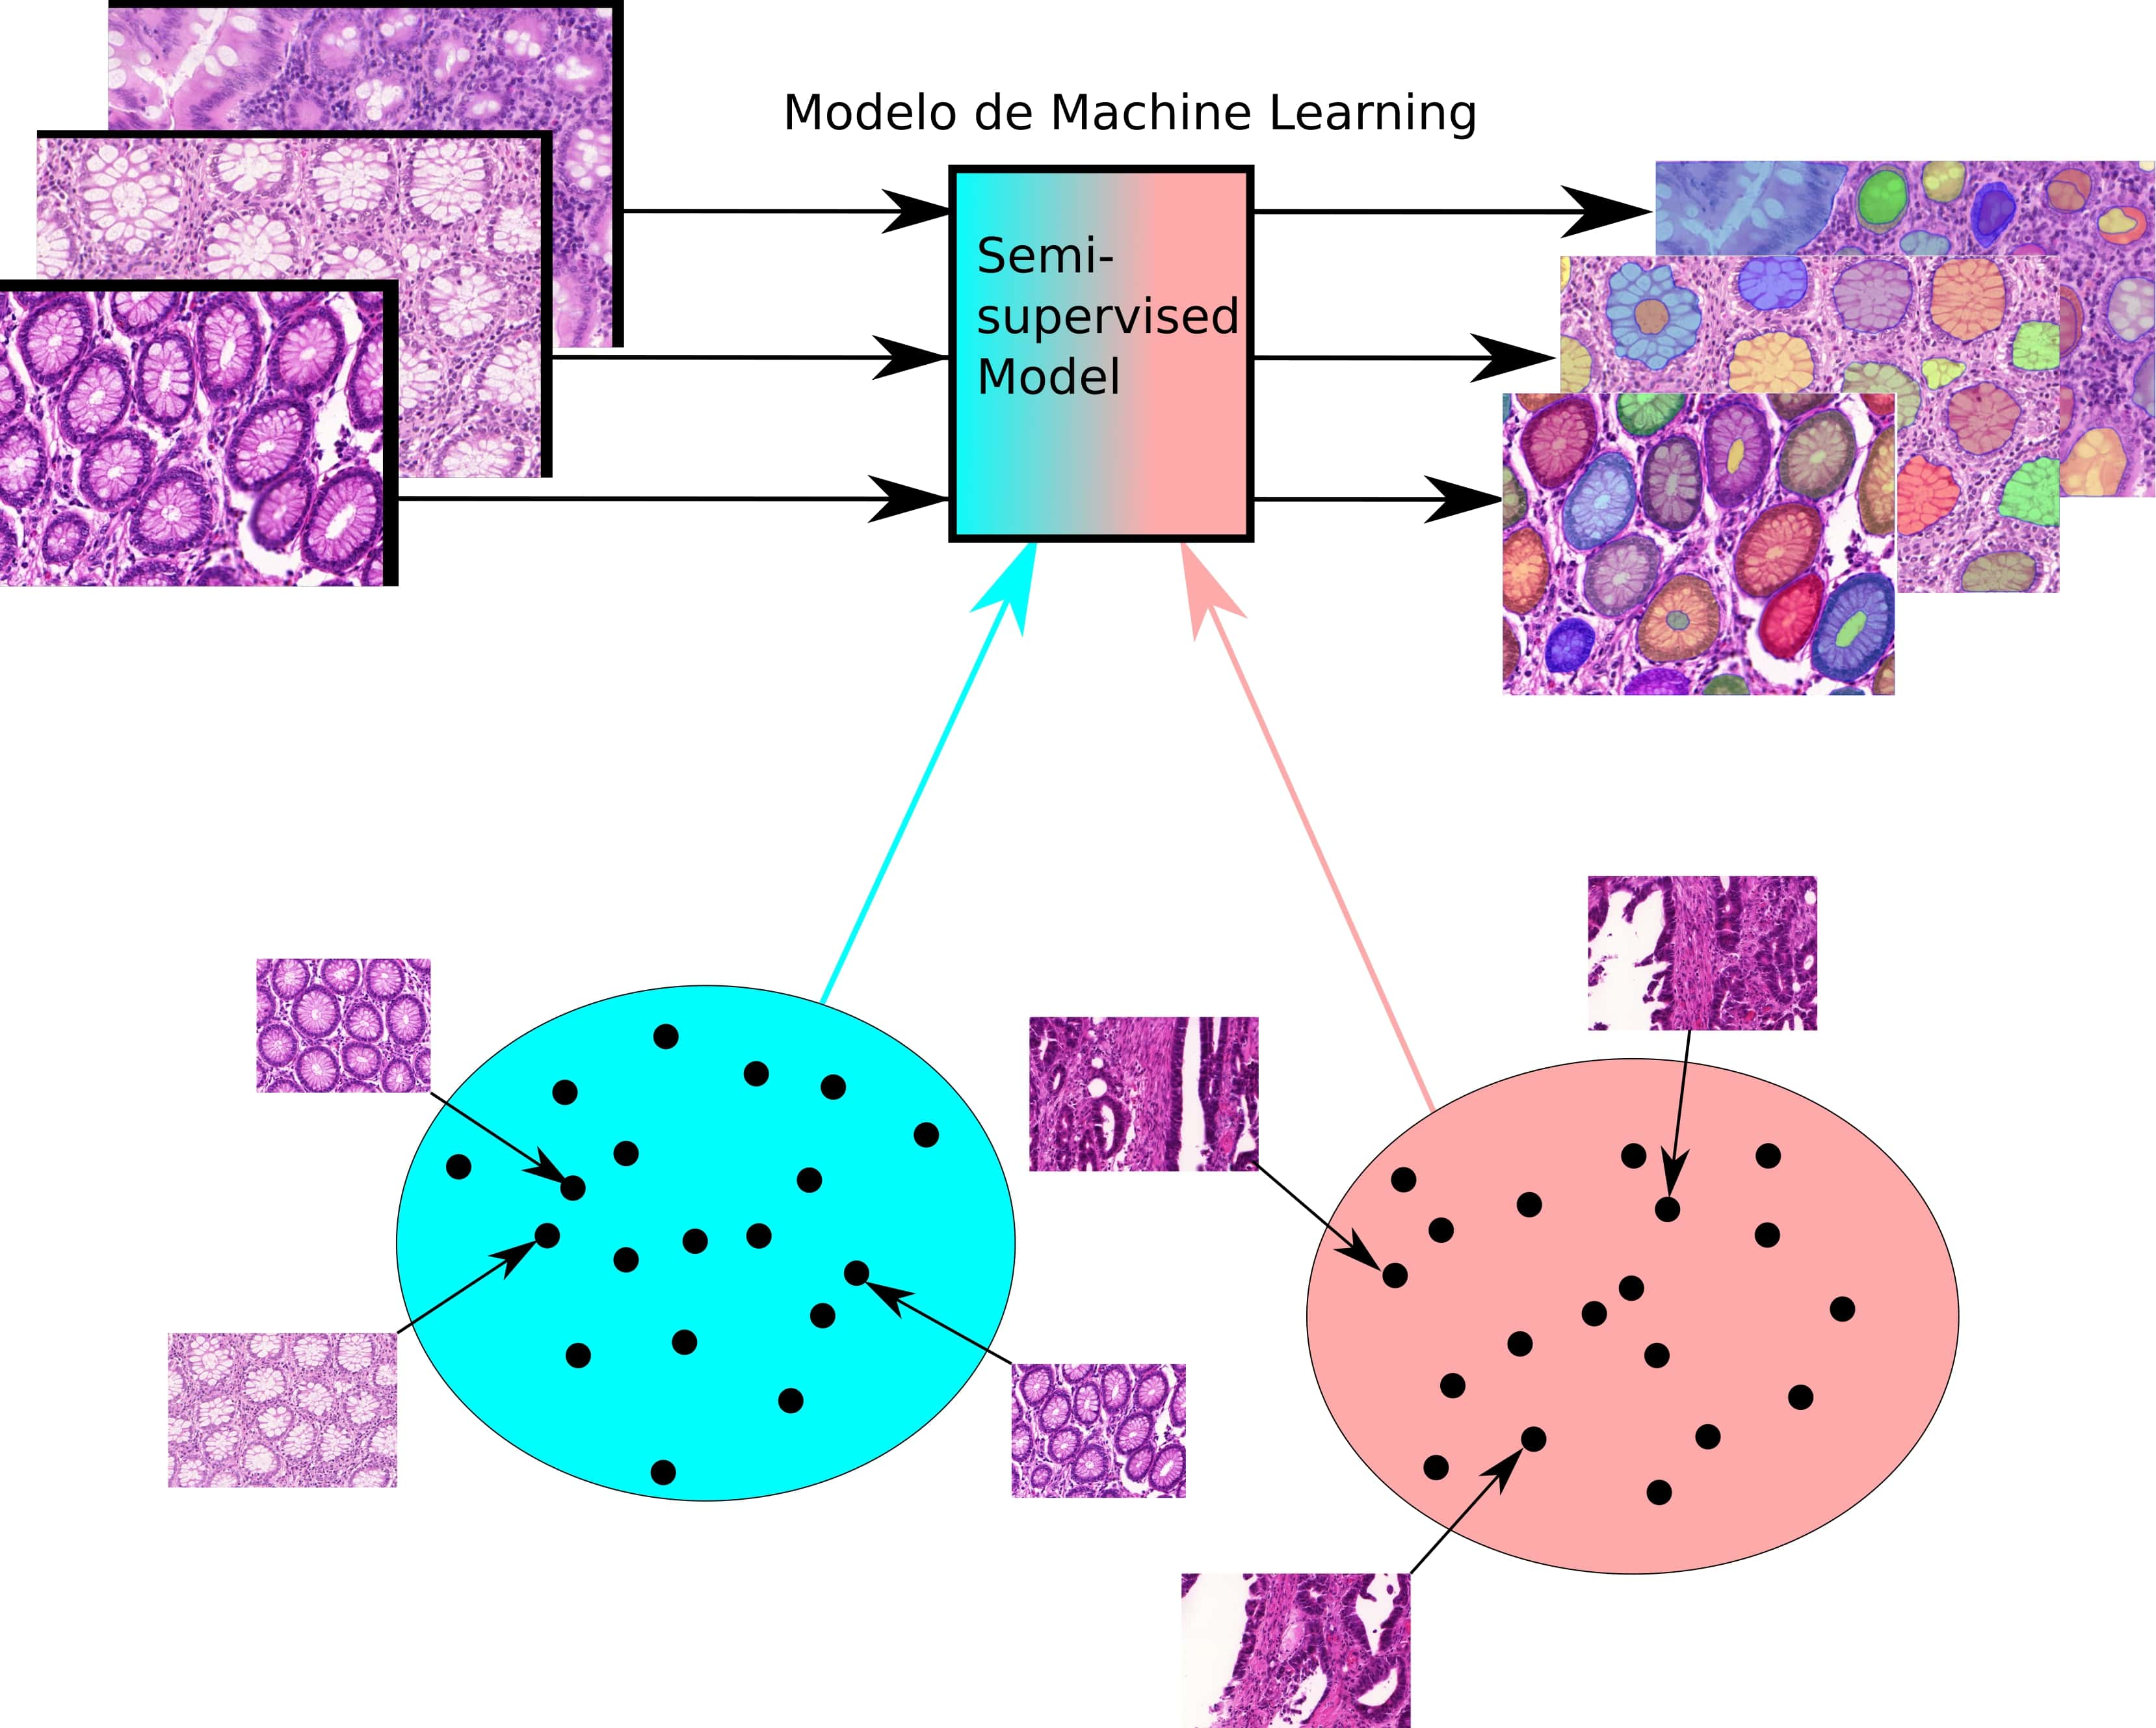
\includegraphics[width=\textwidth]{semi_supervised_model.jpg}
    \caption{Esquema semisupervisado en el que una representación aprendida
    con datos sin anotar se reutiliza en una tarea que dispone de etiquetas.}
    \label{fig:semi-supervised}
\end{figure}
\section{Redes neuronales profundas}

Una red neuronal profunda compone transformaciones afines con funciones no
lineales. En una capa densa, una entrada \(\mathbf x\in\mathbb R^{d_{in}}\)
se transforma como \(\mathbf y=\phi(\mathbf W\mathbf x+\mathbf b)\), con
\(\mathbf W\in\mathbb R^{d_{out}\times d_{in}}\),
\(\mathbf b\in\mathbb R^{d_{out}}\) y una no linealidad \(\phi\). Durante el
entrenamiento, la diferenciación inversa proporciona los gradientes usados por
un optimizador para reducir una función de pérdida
~\cite{goodfellow_deep_2016}. La Figura~\ref{fig:deep_nets} muestra una
composición de varias capas.
\begin{figure}[h!]
    \centering
    
\includegraphics[width=0.9\textwidth]{neural_nets.drawio.jpg}
    \caption{Ejemplo de una red neuronal profunda. Cada capa oculta aplica una
    transformación afín y una no linealidad; la capa de salida produce la
    predicción correspondiente a la tarea.}
    \label{fig:deep_nets}
\end{figure}

Las redes neuronales convolucionales (CNN) sustituyen parte de las matrices
densas por núcleos locales cuyos coeficientes se comparten entre posiciones.
En imágenes, esta estructura reduce el número de parámetros y conserva la
organización espacial. La operación puede entenderse como el desplazamiento de
un filtro sobre una cuadrícula, como se ilustra en la
Figura~\ref{fig:convolution}.
\begin{figure}[h!]
    \centering
    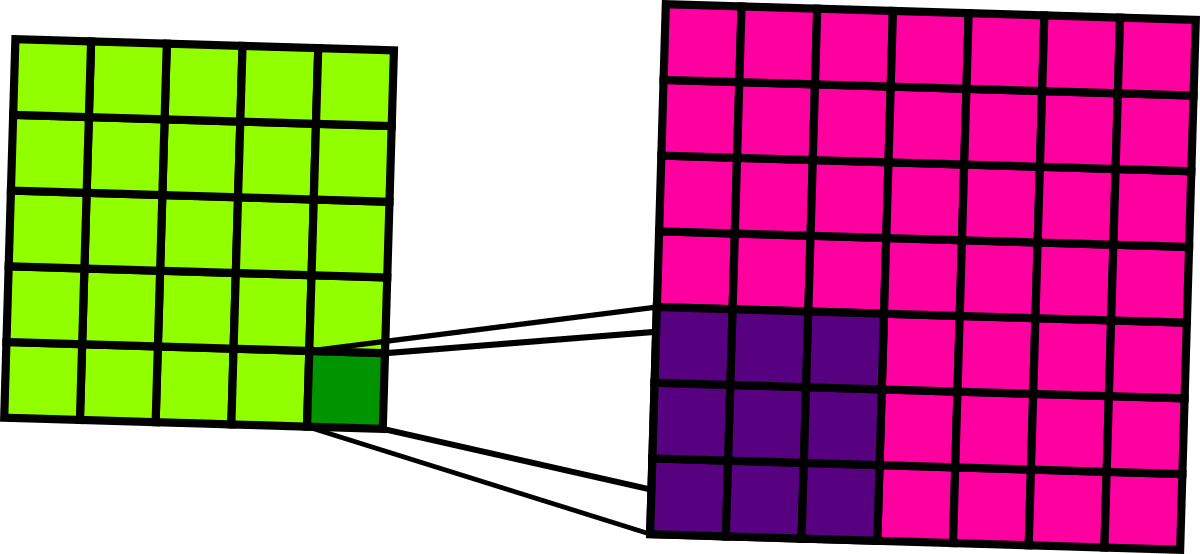
\includegraphics[width=0.6\textwidth]{convolution_classical.png}
    \caption{Ejemplo de convolución discreta para un filtro que se desliza sobre la grilla magenta. La función del filtro la transforma a otro valor (color verde). Se puede ver que el proceso es local: solo se toman elementos que conforman un vecindario en la grilla para generar el resultado.}
\label{fig:convolution}
\end{figure}


Para funciones \(f,g:\mathbb R\rightarrow\mathbb R\), la convolución continua
se define por

\begin{equation}
(f * g)(x) = \int_{-\infty}^{\infty} f(t)g(x-t)\,dt .
\end{equation}


Para secuencias \(f,g:\mathbb Z\rightarrow\mathbb R\), la integral se
reemplaza por una suma:
\begin{equation}
(f * g)[n] = \sum_{m=-\infty}^{\infty} f[m]g[n-m] .
\end{equation}

Las bibliotecas de aprendizaje profundo suelen implementar correlación cruzada,
sin invertir el núcleo; como los coeficientes se aprenden, se conserva la misma
capacidad de representación y se mantiene el nombre de convolución por
convención~\cite{goodfellow_deep_2016}. Una convolución con paso unitario es
equivariante a traslaciones en el dominio ideal: trasladar la entrada traslada
la salida. Esta propiedad no significa invariancia y puede dejar de ser exacta
en bordes o cuando se introducen relleno, submuestreo o agrupamiento
~\cite{cohen_group_2016}. La misma distinción entre equivarianza e invariancia
será utilizada para las rotaciones.


\section{Aprendizaje de instancias múltiples y atención espacial}

En una WSI, la etiqueta clínica describe la lámina completa, aunque el tejido
se procese como miles de parches que no tienen una etiqueta diagnóstica
individual. El aprendizaje de instancias múltiples (MIL, por sus siglas en
inglés) representa esta situación mediante una bolsa de instancias y una sola
etiqueta para la bolsa. En el MIL de atención, cada parche se transforma en un
vector y una función invariante a permutaciones aprende cuánto aporta a la
representación global~\cite{ilse_attention_2018}. En patología computacional,
CLAM complementa esa agregación con agrupamiento de instancias y supervisión
débil~\cite{lu_dataefficient_2021}, mientras DSMIL combina evidencia de una
instancia crítica con una representación agregada de la bolsa
~\cite{li_dualstream_2021}.

La operación central de un Transformer es la atención de producto punto
escalado~\cite{vaswani_attention_2017}. Sean una secuencia de consultas
\(\mathbf X_q\in\mathbb R^{n_q\times d}\) y una secuencia que aporta claves y
valores \(\mathbf X_{kv}\in\mathbb R^{n_k\times d}\). Para una cabeza de
atención, tres transformaciones afines producen

\begin{equation}
    \begin{aligned}
    \mathbf Q&=\mathbf X_q\mathbf W_Q+\mathbf 1\mathbf b_Q^{\mathsf T}
        \in\mathbb R^{n_q\times d_k},\\
    \mathbf K&=\mathbf X_{kv}\mathbf W_K+\mathbf 1\mathbf b_K^{\mathsf T}
        \in\mathbb R^{n_k\times d_k},\\
    \mathbf V&=\mathbf X_{kv}\mathbf W_V+\mathbf 1\mathbf b_V^{\mathsf T}
        \in\mathbb R^{n_k\times d_v},
    \end{aligned}
    \label{eq:qkv-transformer}
\end{equation}

donde, por ejemplo, \(\mathbf W_Q\in\mathbb R^{d\times d_k}\) y
\(\mathbf b_Q\in\mathbb R^{d_k}\). La atención propia toma
\(\mathbf X_q=\mathbf X_{kv}\); la atención cruzada conserva las dos secuencias
distintas. Cada fila de \(\mathbf Q\mathbf K^{\mathsf T}\) compara una consulta
con todas las claves. Para un vector \(\mathbf s\in\mathbb R^{m}\), se define

\begin{equation}
    \operatorname{softmax}(\mathbf s)_j
    =\frac{\exp(s_j-s_{\max})}
    {\sum_{l=1}^{m}\exp(s_l-s_{\max})},
    \qquad s_{\max}=\max_l s_l .
    \label{eq:definicion-softmax}
\end{equation}

La resta de \(s_{\max}\) no cambia el resultado y evita exponenciales
innecesariamente grandes. Aplicada a cada fila, esta función produce pesos no
negativos cuya suma es uno. La salida de una cabeza es

\begin{equation}
    \operatorname{Attn}(\mathbf Q,\mathbf K,\mathbf V;\mathbf M)
    =\operatorname{softmax}_{\mathrm{fila}}\!\left(
        \frac{\mathbf Q\mathbf K^{\mathsf T}}{\sqrt{d_k}}+\mathbf M
      \right)\mathbf V
    \in\mathbb R^{n_q\times d_v}.
    \label{eq:atencion-producto-punto}
\end{equation}

La matriz \(\mathbf M\in(\mathbb R\cup\{-\infty\})^{n_q\times n_k}\)
permite añadir sesgos o excluir conexiones: después de \emph{softmax}, una
entrada con valor \(-\infty\) recibe peso cero. El factor \(\sqrt{d_k}\)
controla la escala de los productos internos. En atención de múltiples cabezas
(MHA, \emph{multi-head attention}), cada cabeza \(h\in\{1,\ldots,H\}\)
posee proyecciones propias y calcula \(\mathbf A_h\) mediante la
Ecuación~\eqref{eq:atencion-producto-punto}. Sus salidas se concatenan y se
mezclan con una proyección final:

\begin{equation}
    \operatorname{MHA}(\mathbf X_q,\mathbf X_{kv})
    =\operatorname{concat}(\mathbf A_1,\ldots,\mathbf A_H)\mathbf W_O
     +\mathbf 1\mathbf b_O^{\mathsf T}
    \in\mathbb R^{n_q\times d},
    \label{eq:definicion-mha}
\end{equation}

donde usualmente \(d_k=d_v=d_h=d/H\), de modo que la concatenación tiene
ancho \(Hd_h=d\), \(\mathbf W_O\in\mathbb R^{d\times d}\) y
\(\mathbf b_O\in\mathbb R^d\). Para simplificar la notación se escribe
\(\operatorname{MHA}(\mathbf X)\) cuando se trata de atención propia.

La normalización por capas (LN, \emph{layer normalization}) se aplica a cada
token por separado~\cite{ba_layernorm_2016}. Para la fila
\(\mathbf x_i\in\mathbb R^d\),

\begin{equation}
    \begin{gathered}
    \mu_i=\frac{1}{d}\sum_{r=1}^{d}x_{ir},\qquad
    \nu_i=\frac{1}{d}\sum_{r=1}^{d}(x_{ir}-\mu_i)^2,\\
    \operatorname{LN}(\mathbf x_i)_r
      =\gamma_r\frac{x_{ir}-\mu_i}{\sqrt{\nu_i+\epsilon}}+\beta_r,
      \qquad \boldsymbol\gamma,\boldsymbol\beta\in\mathbb R^d.
    \end{gathered}
    \label{eq:definicion-layernorm}
\end{equation}

Los vectores \(\boldsymbol\gamma\) y \(\boldsymbol\beta\) son aprendidos y
\(\epsilon>0\) evita dividir por cero. En los bloques pre-normalizados, LN se
evalúa antes de cada rama y su salida se suma al estado que entró a la rama
~\cite{xiong_layernorm_2020}.
La segunda rama emplea SwiGLU~\cite{shazeer_glu_2020}. Si
\(\mathbf Z=\operatorname{LN}(\mathbf U)\in\mathbb R^{n\times d}\), esta
unidad se define como

\begin{equation}
    \begin{aligned}
    \sigma(a)&=\frac{1}{1+e^{-a}},\qquad
    \operatorname{SiLU}(a)=a\,\sigma(a),\\
    \operatorname{SwiGLU}(\mathbf Z)
      &=\left[\operatorname{SiLU}(\mathbf Z\mathbf W_g+\mathbf b_g)
      \odot(\mathbf Z\mathbf W_v+\mathbf b_v)\right]\mathbf W_2+\mathbf b_2.
    \end{aligned}
    \label{eq:definicion-swiglu}
\end{equation}

Aquí \(\mathbf W_g,\mathbf W_v\in\mathbb R^{d\times d_{ff}}\),
\(\mathbf W_2\in\mathbb R^{d_{ff}\times d}\), los sesgos tienen los anchos
correspondientes y \(\odot\) denota multiplicación elemento a elemento. Un
bloque Transformer pre-normalizado completo queda entonces

\begin{equation}
    \mathbf U=\mathbf X+\operatorname{MHA}(\operatorname{LN}_1(\mathbf X)),
    \qquad
    \mathbf Y=\mathbf U+\operatorname{SwiGLU}(\operatorname{LN}_2(\mathbf U)).
    \label{eq:bloque-transformer-prenorm}
\end{equation}

Las dos sumas residuales conservan la forma \(n\times d\). Cuando no se
agregan posiciones absolutas y todas las filas se permutan conjuntamente, la
atención es equivariante a esa permutación. Una o varias consultas aprendidas
pueden entonces resumir el conjunto en un número fijo de vectores, idea
relacionada con el agrupamiento por atención del Set
Transformer~\cite{lee_settransformer_2019}. Esto permite tratar una WSI como
una bolsa cuyo número de parches varía entre láminas.

Tratar la WSI únicamente como un conjunto elimina, sin embargo, la vecindad que
existe entre parches contiguos. La atención sobre grafos permite restringir las
interacciones a las aristas de un grafo local~\cite{velickovic_graph_2018}. En
visión, arquitecturas como Swin y Neighborhood Attention muestran que usar
ventanas o vecindarios móviles conserva contexto espacial con crecimiento
lineal respecto del número de elementos~\cite{liu_swin_2021,hassani_neighborhood_2023}.
En atención por ventanas se particiona la cuadrícula en conjuntos disjuntos
\(\Omega_1,\ldots,\Omega_R\) de \(w\) posiciones y se emplea la máscara

\begin{equation}
    M^{\mathrm{win}}_{ij}=
    \begin{cases}
       0, & \text{si existe }r\text{ tal que }i,j\in\Omega_r,\\
       -\infty, & \text{en otro caso}.
    \end{cases}
    \label{eq:mascara-window-attention}
\end{equation}

Por tanto, la matriz de atención es diagonal por bloques y su costo es
\(\sum_r|\Omega_r|^2=nw\) cuando el tamaño de ventana es fijo, en vez de
\(n^2\). Swin desplaza la partición entre bloques para comunicar ventanas
adyacentes, mientras Neighborhood Attention centra una vecindad móvil en cada
consulta. La Figura~\ref{fig:atencion-ventanas-mapa} muestra la diferencia
entre la matriz global y la máscara local.

\begin{figure}[htbp]
    \centering
    \resizebox{0.92\textwidth}{!}{\begin{tikzpicture}[
    font=\sffamily\scriptsize,
    >={Latex[length=2.8mm]},
    flow/.style={->,very thick,draw=black!70},
    title/.style={font=\sffamily\small\bfseries,align=center},
    note/.style={align=center,text=black!75}
]
% Spatial tokens and a fixed two-window partition.
\node[title] at (2.0,2.85) {cuadrícula de tokens};
\foreach \row in {0,1}{
  \foreach \col in {0,1,2,3}{
    \pgfmathtruncatemacro{\token}{4*\row+\col+1}
    \ifnum\col<2
      \def\cellcolor{blue!18}
    \else
      \def\cellcolor{orange!20}
    \fi
    \draw[fill=\cellcolor,draw=black!55,line width=0.7pt]
      (\col,1-\row) rectangle ++(1,1);
    \node at (\col+0.5,1.5-\row) {$x_{\token}$};
  }
}
\draw[red!75!black,line width=2.1pt] (0,1) rectangle ++(1,1);
\node[note] at (2.0,-0.48) {dos ventanas de cuatro tokens;\\$x_1$ es la consulta señalada};

\draw[flow] (4.45,1.0) -- (5.25,1.0);

% Dense attention matrix.
\node[title] at (7.05,2.85) {atención global};
\foreach \i in {0,...,7}{
  \foreach \j in {0,...,7}{
    \pgfmathtruncatemacro{\shade}{12+mod(17*\i+23*\j,72)}
    \draw[fill=blue!\shade,draw=white,line width=0.45pt]
      (5.55+0.38*\j,2.22-0.38*\i) rectangle ++(0.38,-0.38);
  }
}
\draw[red!75!black,line width=1.4pt] (5.55,2.22) rectangle ++(3.04,-0.38);
\node[rotate=90,anchor=south] at (5.18,0.70) {consultas};
\node at (7.07,-1.06) {claves};
\node[note] at (7.07,-1.55) {$8\times8$: cada token compara\\con todos los demás};

\draw[flow] (9.05,1.0) -- (9.85,1.0);

% Block-diagonal window attention map.
\node[title] at (11.68,2.85) {atención por ventanas};
\foreach \i in {0,...,7}{
  \foreach \j in {0,...,7}{
    \pgfmathtruncatemacro{\blocki}{int(\i/4)}
    \pgfmathtruncatemacro{\blockj}{int(\j/4)}
    \ifnum\blocki=\blockj
      \pgfmathtruncatemacro{\shade}{18+mod(19*\i+29*\j,70)}
      \def\cellcolor{blue!\shade}
    \else
      \def\cellcolor{black!8}
    \fi
    \draw[fill=\cellcolor,draw=white,line width=0.45pt]
      (10.16+0.38*\j,2.22-0.38*\i) rectangle ++(0.38,-0.38);
  }
}
\draw[red!75!black,line width=1.4pt] (10.16,2.22) rectangle ++(3.04,-0.38);
\draw[black!65,line width=1pt] (10.16,2.22) rectangle ++(1.52,-1.52);
\draw[black!65,line width=1pt] (11.68,0.70) rectangle ++(1.52,-1.52);
\node[rotate=90,anchor=south] at (9.79,0.70) {consultas};
\node at (11.68,-1.06) {claves};
\node[note] at (11.68,-1.55) {bloques activos: pesos locales;\\gris: conexiones enmascaradas};

% Weight legend.
\foreach \k in {0,...,7}{
  \pgfmathtruncatemacro{\shade}{8+11*\k}
  \fill[blue!\shade] (13.75+0.24*\k,1.34) rectangle ++(0.24,0.28);
}
\draw[black!45] (13.75,1.34) rectangle ++(1.92,0.28);
\node[anchor=north west] at (13.70,1.22) {peso bajo};
\node[anchor=north east] at (15.72,1.22) {alto};
\node[note,text width=2.2cm] at (14.72,0.10)
    {cada fila se normaliza por separado};
\end{tikzpicture}
}
    \caption{Atención global y atención por ventanas. Cada fila de la matriz
    representa una consulta y cada columna una clave; el color representa el
    peso después de \emph{softmax}. Al restringir la atención, las entradas
    fuera de la ventana reciben \(-\infty\) antes de normalizar y quedan en
    cero. La consulta marcada en la cuadrícula solo combina los valores de su
    región local. Elaboración propia.}
    \label{fig:atencion-ventanas-mapa}
\end{figure}

Otros modelos introducen convoluciones en la formación de tokens y en las
proyecciones de atención para recuperar sesgos locales propios de las
imágenes~\cite{wu_cvt_2021}. Estas ideas no determinan una única arquitectura,
pero motivan separar una etapa local, que relaciona parches vecinos, de otra
global, que resume la WSI completa.

La forma habitual de atención normaliza las puntuaciones mediante
\emph{softmax}. También es posible usar compuertas sigmoides independientes,
siempre que se controle su escala al cambiar la longitud de la secuencia. El
análisis de Ramapuram et al. muestra que una atención sigmoidal correctamente
normalizada puede igualar el comportamiento de \emph{softmax} en diversos
dominios y destaca la necesidad de estabilizar su masa inicial
~\cite{ramapuram_sigmoid_2025}. Esta distinción resulta relevante para bolsas
de WSI cuyo número de parches puede variar en varios órdenes de magnitud.




\section{Redes neuronales convolucionales equivariantes}

Una convolución ordinaria comparte el mismo núcleo en todas las posiciones y,
salvo efectos de borde o submuestreo, es equivariante a traslaciones. Si una
entrada se desplaza, el mapa de características se desplaza de la misma forma;
la salida no permanece necesariamente fija~\cite{cohen_group_2016,lim_what_2022}.
Rotaciones y reflexiones son acciones diferentes y una CNN ordinaria no es
equivariante a ellas por construcción. La Figura~\ref{fig:cat} muestra estas
transformaciones en una imagen natural y en un recorte histológico.
\begin{figure}[h!]

\includegraphics[width=1\textwidth]{transformaciones_gato_wsi.png}
\caption{Ejemplos de traslación, rotación y reflexión aplicadas a una imagen
natural y a un recorte histológico.}
\label{fig:cat}
\end{figure}


La salida deseada determina si la transformación debe producir invariancia o
equivarianza. En clasificación, la clase puede permanecer fija; en
segmentación, la máscara debe transformarse junto con la entrada, como se
resume en la Figura~\ref{fig:cat_segmentation}.

\begin{figure}[h!]
\centering
\subcaptionbox{Invarianza}{
\includegraphics[width=0.35\linewidth]{fig2.jpg}}
\quad
\subcaptionbox{Equivarianza}{
\includegraphics[width=0.55
\linewidth]{fig3.jpg}}
\caption{En \textbf{(a)} se muestra cómo la clasificación puede ser invariante.
    En \textbf{(b)} se muestra cómo la segmentación puede ser equivariante.}
\label{fig:cat_segmentation}
\end{figure}


En histopatología, la orientación del tejido sobre el portaobjetos no define por
sí sola la clase diagnóstica. Esta observación ha motivado modelos que comparten
filtros entre rotaciones y reflexiones en tareas histológicas
~\cite{veeling_rotation_2018}. No toda imagen presenta esta simetría: los
dígitos \(6\) y \(9\), por ejemplo, pueden intercambiar su identidad al rotarse
\(180^\circ\), como ilustra la Figura~\ref{fig:69}.

\begin{figure}[h!]
    \centering
    
\includegraphics[width=0.3\textwidth]{6.jpg}
    
\includegraphics[width=0.3\textwidth]{9.jpg}
    \caption{Ejemplo de una tarea que no posee invariancia rotacional: una
    rotación de \(180^\circ\) puede intercambiar los dígitos 6 y 9.}
    \label{fig:69}
\end{figure}
Como en las CNN usuales, aprovechar una simetría introduce un sesgo inductivo
y permite compartir parámetros sobre las transformaciones consideradas
~\cite{cesa_program_2021}. El aumento de datos
ofrece otra forma de exponer el modelo a transformaciones geométricas. Bajo
supuestos específicos sobre la distribución, la función objetivo y la clase
de modelos, se han demostrado beneficios de generalización para imponer
equivarianza directamente \cite{elesedy_provably_2021}; esto no garantiza una
ventaja en todo conjunto de datos y debe contrastarse empíricamente en el
presente estudio.
\paragraph{Grupos y acciones.}

Un grupo \(G\) es un conjunto dotado de una operación interna. Para
\(a,b,c\in G\), esta operación es asociativa, existe una identidad \(e\) y
cada elemento posee un inverso~\cite{hall_lie_groups_2015}:

\begin{equation}
    (ab)c=a(bc),\qquad ea=ae=a,\qquad a^{-1}a=aa^{-1}=e.
    \label{eq:axiomas-grupo}
\end{equation}

Una acción especifica cómo cada \(g\in G\) transforma un espacio. En espacios
vectoriales se representa mediante operadores lineales invertibles
\(\rho(g)\), con \(\rho(e)=\mathbf I\) y
\(\rho(g_1g_2)=\rho(g_1)\rho(g_2)\). En este trabajo, el grupo incorporado es
el de rotaciones continuas del plano,

\begin{equation}
    \mathrm{SO}(2)=\left\{\mathbf R_\theta=
    \begin{bmatrix}\cos\theta&-\sin\theta\\
                    \sin\theta& \cos\theta\end{bmatrix}:
    \theta\in[0,2\pi)\right\}.
    \label{eq:definicion-so2}
\end{equation}

No se incorporaron reflexiones. Una red equivariante codifica esta acción en
sus capas; el aumento de datos, en cambio, presenta ejemplos transformados
durante el ajuste.

\paragraph{Mapas equivariantes.}

Sean \(X\) y \(Y\) los espacios de entrada y salida, con representaciones
posiblemente distintas \(\rho_X\) y \(\rho_Y\). Una función
\(F:X\rightarrow Y\) es equivariante a \(G\) si

\begin{equation}
    F\!\left(\rho_X(g)\mathbf x\right)
    =\rho_Y(g)F(\mathbf x),
    \qquad \forall g\in G,\ \mathbf x\in X.
    \label{eq:definicion-equivarianza}
\end{equation}

Las dos rutas de la Ecuación~\eqref{eq:definicion-equivarianza} forman el
diagrama conmutativo siguiente.
\begin{center}

\includegraphics[scale=0.1]{equivariance_diagram.jpg}
\end{center}
\paragraph{Convolución en grupos.}

La convolución puede extenderse a señales definidas sobre un grupo. Sean
\(\mathbf f:G\rightarrow\mathbb R^{c_{in}}\) una señal y
\(\boldsymbol\psi:G\rightarrow
\mathbb R^{c_{out}\times c_{in}}\) un núcleo. Se define

\begin{equation}
    (\mathbf f*\boldsymbol\psi)(x)
    =\int_G \boldsymbol\psi(y^{-1}x)\,\mathbf f(y)\,d\lambda(y)
    \in\mathbb R^{c_{out}},
    \label{eq:convolucion-grupo}
\end{equation}

donde \(d\lambda\) es una medida de Haar invariante por la izquierda:
\(\lambda(hA)=\lambda(A)\). En grupos compactos puede normalizarse para que
\(\lambda(G)=1\); en un grupo discreto, la integral se convierte en una suma.
Si \([L_h\mathbf f](x)=\mathbf f(h^{-1}x)\), entonces

\begin{equation}
    L_h(\mathbf f*\boldsymbol\psi)
      =(L_h\mathbf f)*\boldsymbol\psi,
    \label{eq:equivarianza-convolucion-grupo}
\end{equation}

que expresa equivarianza a la acción regular izquierda. Para grupos compactos
y bajo restricciones naturales sobre las capas lineales, Kondor y Trivedi
caracterizan la estructura convolucional como condición necesaria y suficiente
para equivarianza~\cite{kondor_generalization_2018}. La
Figura~\ref{fig:conv_equivariant} ilustra las dos rutas equivalentes.

\begin{figure}[h!]
    \centering
    
\includegraphics[width=0.45\textwidth]{aplicacion_en_f.jpg}
    
\includegraphics[width=0.45\textwidth]{aplicacion_en_fg.jpg}
    \caption{Equivarianza de una convolución respecto de una rotación de
    \(60^\circ\): transformar la entrada antes de la operación produce el
    mismo resultado que transformar la salida.}
    \label{fig:conv_equivariant}
\end{figure}

\begin{figure}[h!]
    \centering
    
\includegraphics[width=0.5\textwidth]{hexagono.jpg}
    \caption{Diagrama ilustrativo de la
    Ecuación~\eqref{eq:equivarianza-convolucion-grupo} para el grupo discreto
    de rotaciones de un hexágono.}
    \label{fig:convdiagram}
\end{figure}

\section{Trabajos relacionados}


Los trabajos relacionados pueden agruparse en tres líneas: convoluciones
equivariantes generales, aplicaciones en imágenes médicas y regularización de
espacios latentes. Cohen y Welling introdujeron redes convolucionales sobre
grupos discretos y reportaron errores de 2,28\% en rotated-MNIST y de 4,19\% y
6,46\% en CIFAR-10 con y sin aumento de datos, respectivamente
~\cite{cohen_group_2016}. Posteriormente formularon las CNN direccionables,
en las cuales la restricción de equivarianza se impone sobre el espacio de
núcleos~\cite{cohen_steerable_2016}. Esta línea se apoya en la teoría clásica
de filtros orientables de Freeman y Adelson~\cite{freeman_design_1991}.

Por otra parte, Elesedy \& Zaidi estudian garantías teóricas de generalización
para modelos equivariantes y caracterizan condiciones bajo las cuales imponer
la simetría produce un beneficio estricto frente a estimadores no restringidos
o basados en aumento de datos \cite{elesedy_provably_2021}. La garantía depende
de los supuestos del análisis y no implica que cualquier arquitectura
equivariante supere empíricamente a cualquier línea base. En imágenes, la
equivarianza traslacional conduce a la estructura de las convoluciones
usuales.

La relación entre equivarianza y organización del espacio latente también ha
sido estudiada en autoencodificadores. Kouzelis et al. propusieron EQ-VAE, una
regularización aplicada a autoencodificadores preentrenados para favorecer que
transformaciones semánticamente conservativas, entre ellas la rotación, tengan
una respuesta más sencilla en el latente~\cite{kouzelis_eqvae_2025}. Su método
no emplea convoluciones direccionables y su objetivo final es acelerar modelos
generativos; por tanto, no es equivalente al VAE-\(\mathrm{SO}(2)\) de esta
tesis. Sin embargo, su hipótesis de que un latente equivariante puede tener una
geometría menos compleja motivó parte de las visualizaciones y mediciones
geométricas utilizadas en este trabajo.

Weiler y Cesa obtuvieron soluciones analíticas para espacios de núcleos
equivariantes a \(E(2)\) y las implementaron en una biblioteca de PyTorch
~\cite{weiler_general_2019}. Cesa et al. extendieron el teorema de
Wigner--Eckart para parametrizar núcleos direccionables sobre espacios de
grupos compactos y reunieron estas construcciones en el programa
\texttt{escnn}~\cite{cesa_program_2021}. En una dirección complementaria,
Weiler et al. presentaron una formulación libre de coordenadas para
convoluciones equivariantes a isometrías y cambios de marco en variedades
riemannianas, con una demostración sobre una banda de Möbius
~\cite{weiler_coordinate_2021}.

En imágenes médicas, Bekkers et al. estudiaron convoluciones covariantes a
rotaciones y traslaciones de \(\mathrm{SE}(2)\), sin incluir reflexiones, en
tres tareas: detección de mitosis, segmentación de vasos retinianos y
segmentación de células~\cite{bekkers_roto-translation_2018}. Sus experimentos
compararon varias discretizaciones angulares y mostraron el efecto de aumentar
la resolución del muestreo de rotaciones. Veeling et al. evaluaron redes
equivariantes al grupo \(p4m\), que incorpora rotaciones de múltiplos de
\(90^\circ\) y reflexiones, para detectar metástasis en parches de ganglio
linfático; frente a su línea base reportaron mejor exactitud y eficiencia de
parámetros~\cite{veeling_rotation_2018}. Li et al. combinaron filtros dinámicos
con convoluciones equivariantes y reportaron mejoras frente a las líneas base
consideradas en tareas de imagen médica~\cite{li_dynamic_2020}.
Estos antecedentes muestran que existen métodos equivariantes para
clasificación supervisada, pero que la utilidad de ese sesgo inductivo en un
autoencodificador histopatológico debe evaluarse de manera separada. En esta
tesis se estudió esa relación mediante reconstrucción, tareas supervisadas con
representaciones congeladas y análisis de la respuesta latente a rotaciones,
sin asumir de antemano que la restricción geométrica produciría una ventaja en
todas las medidas.
